%%%%%%%%%%%%%%%%%%%%%%%%%%%%%%%%%%%%%%%%%
% Beamer Presentation
% LaTeX Template
% Version 1.0 (10/11/12)
%
% This template has been downloaded from:
% http://www.LaTeXTemplates.com
%
% License:
% CC BY-NC-SA 3.0 (http://creativecommons.org/licenses/by-nc-sa/3.0/)
%
%%%%%%%%%%%%%%%%%%%%%%%%%%%%%%%%%%%%%%%%%

%----------------------------------------------------------------------------------------
%	PACKAGES AND THEMES
%----------------------------------------------------------------------------------------

\documentclass[handout]{beamer}

\mode<presentation> {

% The Beamer class comes with a number of default slide themes
% which change the colors and layouts of slides. Below this is a list
% of all the themes, uncomment each in turn to see what they look like.

%\usetheme{default}
%\usetheme{AnnArbor}
%\usetheme{Antibes}
%\usetheme{Bergen}
%\usetheme{Berkeley}
%\usetheme{Berlin}
%\usetheme{Boadilla}
%\usetheme{CambridgeUS}
%\usetheme{Copenhagen}
%\usetheme{Darmstadt}
%\usetheme{Dresden}
%\usetheme{Frankfurt}
%\usetheme{Goettingen}
%\usetheme{Hannover}
%\usetheme{Ilmenau}
%\usetheme{JuanLesPins}
%\usetheme{Luebeck}
\usetheme{Madrid}
%\usetheme{Malmoe}
%\usetheme{Marburg}
%\usetheme{Montpellier}
%\usetheme{PaloAlto}
%\usetheme{Pittsburgh}
%\usetheme{Rochester}
%\usetheme{Singapore}
%\usetheme{Szeged}
%\usetheme{Warsaw}

% As well as themes, the Beamer class has a number of color themes
% for any slide theme. Uncomment each of these in turn to see how it
% changes the colors of your current slide theme.

%\usecolortheme{albatross}
%\usecolortheme{beaver}
%\usecolortheme{beetle}
%\usecolortheme{crane}
%\usecolortheme{dolphin}
%\usecolortheme{dove}
%\usecolortheme{fly}
%\usecolortheme{lily}
%\usecolortheme{orchid}
%\usecolortheme{rose}
%\usecolortheme{seagull}
%\usecolortheme{seahorse}
%\usecolortheme{whale}
%\usecolortheme{wolverine}

%\setbeamertemplate{footline} % To remove the footer line in all slides uncomment this line
%\setbeamertemplate{footline}[page number] % To replace the footer line in all slides with a simple slide count uncomment this line

%\setbeamertemplate{navigation symbols}{} % To remove the navigation symbols from the bottom of all slides uncomment this line
}

\usepackage{graphicx} % Allows including images
\usepackage{booktabs} % Allows the use of \toprule, \midrule and \bottomrule in tables
\usepackage{cool}
\usepackage{tikz}
\usepackage{amsmath}
\usepackage{xcolor}
\usepackage{hyperref}

\DeclareMathOperator*{\argmax}{argmax}
\DeclareMathOperator*{\argmin}{argmin}
\usetikzlibrary{positioning}

%----------------------------------------------------------------------------------------
%	TITLE PAGE
%----------------------------------------------------------------------------------------

\title[``RL for Finance'' course]{CME 241: Foundations of Reinforcement Learning \\ with Applications in Finance} % The short title appears at the bottom of every slide, the full title is only on the title page

\author{Ashwin Rao} % Your name
\institute[Stanford] % Your institution as it will appear on the bottom of every slide, may be shorthand to save space
{ICME, Stanford University
 % Your institution for the title page
}

\date{Winter 2022} % Date, can be changed to a custom date

\begin{document}
\begin{frame}
\titlepage % Print the title page as the first slide
\end{frame}

% \begin{frame}
% \frametitle{Overview} % Table of contents slide, comment this block out to remove it
% \tableofcontents % Throughout your presentation, if you choose to use \section{} and \subsection{} commands, these will automatically be printed on this slide as an overview of your presentation
% \end{frame}

\begin{frame}
\frametitle{Meet your Instructor}
\pause
\begin{itemize}[<+->]
\item Joined Stanford ICME as Adjunct Professor in Fall 2018
\item Research Interests: A.I. for Dynamic Decisioning under Uncertainty
\item Technical mentor to ICME students, partnerships with industry
\item Educational background: Algorithms Theory \& Abstract Algebra
\item 10 years at Goldman Sachs (NY) {\em Rates/Mortgage Derivatives} Trading
\item 4 years at Morgan Stanley as {\em Managing Director - Market Modeling}
\item Founded Tech Startup {\em ZLemma}, Acquired by hired.com in 2015
\item One of our products was algorithmic jobs/career guidance for students
\item Teaching experience: Pure \& Applied Math, CompSci, Finance, Mgmt
\end{itemize}
\end{frame}


\begin{frame}
\frametitle{Requirements and Setup}
\pause
\begin{itemize}[<+->]
\item Pre-requisites:
\begin{itemize}
\item Undergraduate-level background in Applied Mathematics (Multivariate Analysis, Linear Algebra, Probability, Optimization)
\item Background in data structures/algorithms, fluency with numpy
\item Basic familiarity with Pricing, Portfolio Mgmt and Algo Trading, but we will do an overview of the requisite Finance/Economics
\item No background required in MDP, DP, RL (we will cover from scratch)
\end{itemize}
\item Here's \href{http://web.stanford.edu/class/cme241/lecture_slides/final-2021.pdf}{\underline{\textcolor{blue}{last year's final exam}}}  to get a sense of course difficulty
\item Register for the \href{https://edstem.org/us/courses/16175}{\underline{\textcolor{blue}{course on Ed Discussion}}}
\item Install Python 3 and supporting IDE/tools (eg: PyCharm, Jupyter)
\item Install LaTeX/Markdown and supporting editor for tech writing
\item Download  \href{https://stanford.edu/~ashlearn/RLForFinanceBook/book.pdf}{\underline{\textcolor{blue}{the textbook for this course}}}
\item Assignments and code in the textbook based on \href{https://github.com/TikhonJelvis/RL-Book}{\underline{\textcolor{blue}{this open-source code}}}
\item {\em Fork} this repo and \href{http://web.stanford.edu/class/cme241/lecture_slides/assignments/assignment1.pdf}{\underline{\textcolor{blue}{get set up}}} to use this code in assignments
\item Create separate directories for each assignment for CA (\href{mailto:svenl@stanford.edu}{\underline{\textcolor{blue}{Sven Lerner}}}) to review - send Sven your forked repo URL and {\em git push} often
\end{itemize}
\end{frame}


\begin{frame}
\frametitle{Housekeeping}
\pause
\begin{itemize}[<+->]
\item Grade based on:
\begin{itemize}
\item 25\% 48-hour Mid-Term Exam (on Theory, Modeling, Programming)
\item 40\% 48-hour Final Exam (on Theory, Modeling, Programming)
\item 30\% {\em Assignments}: Technical Writing and Programming
\item 5\% {\em Participation:} In Class, on Ed Discussion, during Office Hours
\end{itemize}
\item Lectures: Wed \& Fri 3:15pm-4:45pm. McCullough 115.
\item First two weeks of lecture will be online (\href{https://stanford.zoom.us/j/96275989341?pwd=ZDJ6aTUzelNiRW9ZQkVHZ1BheEZCZz09}{\underline{\textcolor{blue}{zoom link}}})
\item Office Hours 12:30pm-2:30pm Fri (or by appointment) in ICME Mezzanine level, room M05 (within Huang Engg Bldg)
\item You also have the option of joining these Office Hours \href{https://stanford.zoom.us/j/92139204563?pwd=cFgxTjhiQTlpQzAzRks5RDRDcGYydz09}{\underline{\textcolor{blue}{on zoom}}}
\item Course Web Site: \href{http://cme241.stanford.edu}{\underline{\textcolor{blue}{cme241.stanford.edu}}}
\item Ask Questions and engage in Discussions on \href{https://edstem.org/us/courses/16175}{\underline{\textcolor{blue}{Ed Discussion}}}
\item My e-mail: \href{mailto:ashwin.rao@stanford.edu}{\underline{\textcolor{blue}{ashwin.rao@stanford.edu}}}
\end{itemize}
\end{frame}

\begin{frame}
\frametitle{Purpose and Grading of {\em Assignments}}
\pause
\begin{itemize}[<+->]
\item Assignments shouldn't be treated as ``tests'' with right/wrong answer
\item Rather, they should be treated as part of your learning experience
\item You will {\em truly} understand ideas/models/algorithms only when you {\em write down} the Mathematics and the Code precisely
\item Simply reading Math/Code gives you a false sense of understanding
\item Take the initiative to make up your own assignments
\item Especially on topics you feel you don't quite understand
\item Individual assignments won't get a grade and there are no due dates
\item The CA will review once every 2 weeks and provide feedback
\item It will be graded less on correctness and completeness, and more on:
\begin{itemize}
\item Coding and Technical Writing style that is clear and modular
\item Demonstration of curiosity and commitment to learning through the overall body of assignments work
\item Engagement in asking questions and seeking feedback for improvements
\end{itemize}
\end{itemize}
\end{frame}

\begin{frame}
\frametitle{What is {\em Participation} and why does it matter?}
\pause
\begin{itemize}[<+->]
\item {\em Participation} means engagement and interactions
\item With me, with the CA, and with other students
\item In the classroom, or on Ed Discussion, or during Office Hours
\item Come prepared to each class by reading the corresponding chapter
\item Note down what you didn't understand, and ask in class
\item If it's a deeper question, use Ed Discussion or Office Hours time
\item The textbook is in manuscript version - provide feedback on typos and improvements by \href{https://docs.github.com/en/issues/tracking-your-work-with-issues/creating-an-issue}{\underline{\textcolor{blue}{submitting issues}}} in the \href{https://github.com/TikhonJelvis/RL-book}{\underline{\textcolor{blue}{RL-book git repo}}}
\item We want to bring back a vibrant culture of in-person interactions
\item When you get a job, how you work with others matters A LOT!
\item Teachers can teach best when students ask questions
\end{itemize}
\end{frame}


\begin{frame}
\frametitle{Resources}
\pause
\begin{itemize}[<+->]
\item Course based on my new \href{http://stanford.edu/~ashlearn/RLForFinanceBook/book.pdf}{\underline{\textcolor{blue}{RL For Finance book}}}
\item Supplementary/Optional reading:  \href{http://incompleteideas.net/book/the-book-2nd.html}{\underline{\textcolor{blue}{Sutton-Barto's RL book}}}
\item I prepare slides for each lecture (``guided tour'' of respective chapter)
\item A couple of lecture slides are from \href{https://www.davidsilver.uk/teaching/}{\underline{\textcolor{blue}{David Silver's RL course}}}
\item Code in my book based on \href{https://github.com/TikhonJelvis/RL-Book}{\underline{\textcolor{blue}{this open-source code}}}
\item Reading this code as important as the reading of the theory 
\item We will go over some classical papers on the Finance applications
\item Some supplementary/optional papers from Finance/RL
\item All resources organized on the \href{http://cme241.stanford.edu}{\underline{\textcolor{blue}{course web site}}} (``source of truth'')
\end{itemize}
\end{frame}

\begin{frame}
\frametitle{Stanford Honor Code - For Assignments versus Exams}
\pause
\begin{itemize}[<+->]
\item {\em Assignments}: You can discuss solution approaches with other students
\item Because assignments are graded more for effort than correctness
\item Writing (answers/code) should be your own (don't copy/paste)
\item You can invoke the core modules I have written (as instructed)
\item {\em Exams}: You cannot engage in any conversation with other students
\item Write to the CA if a question is unclear
\item Exams are graded on correctness and completeness
\item So {\em don't ask for help} on how to solve exam questions
\item Open-internet Exams: Search for concepts, not answers to exam Qs
\item If you accidentally run into a strong hint/answer, state it honestly
\end{itemize}
\end{frame}


\begin{frame}
\frametitle{A.I. for Dynamic Decisioning under Uncertainty}
\pause
\begin{itemize}[<+->]
\item Let's browse some terms used to characterize this branch of A.I.
\item {\em Stochastic}: Uncertainty in key quantities, evolving over time
\item {\em Optimization}: A well-defined metric to be maximized (``The Goal'')
\item {\em Dynamic}:  Decisions need to be a function of the changing situations
\item {\em Control}: Overpower uncertainty by persistent steering towards goal
\item Jargon overload due to confluence of Control Theory, O.R. and A.I.
\item For language clarity, let's just refer to this area as {\em Stochastic Control}
\item The core framework is called {\em Markov Decision Processes} (MDP)
\item {\em Reinforcement Learning} is a class of algorithms to solve MDPs
\end{itemize}
\end{frame}



\begin{frame}
\frametitle{The MDP Framework}
\includegraphics[width=12cm, height=7cm]{MDP.png}
\end{frame}

\begin{frame}
\frametitle{Components of the MDP Framework}
\pause
\begin{itemize}[<+->]
\item The {\em Agent} and the {\em Environment} interact in a time-sequenced loop
\item {\em Agent} responds to [{\em State}, {\em Reward}] by taking an {\em Action}
\item {\em Environment} responds by producing next step's (random) {\em State}
\item {\em Environment} also produces a (random) scalar denoted as {\em Reward}
\item Each {\em State} is assumed to have the {\em Markov Property}, meaning:
\begin{itemize}
\item Next {\em State/Reward} depends only on Current {\em State} (for a given {\em Action})
\item Current {\em State} captures all relevant information from {\em History}
\item Current {\em State} is a sufficient statistic of the future (for a given {\em Action})
\end{itemize} 
\item Goal of {\em Agent} is to maximize {\em Expected Sum} of all future {\em Reward}s
\item By controlling the ({\em Policy} : {\em State} $\rightarrow$ {\em Action}) function
\item This is a dynamic (time-sequenced control) system under uncertainty
\end{itemize}
\end{frame}

\begin{frame}
\frametitle{Formal MDP Framework}
The following notation is for discrete time steps. Continuous-time formulation is analogous (often involving
\href{https://github.com/coverdrive/technical-documents/blob/master/finance/cme241/StochasticCalculusFoundations.pdf}{\underline{\textcolor{blue}{Stochastic Calculus}}})
\pause
\begin{itemize}[<+->]
\item Time steps denoted as $t = 1, 2, 3, \ldots$
\item Markov States $S_t \in \mathcal{S}$ where $\mathcal{S}$ is the State Space
\item Actions $A_t \in \mathcal{A}$ where $\mathcal{A}$ is the Action Space
\item Rewards $R_t \in \mathbb{R}$ denoting numerical feedback\
\item Transitions $p(r,s'|s,a) = \mathbb{P}[(R_{t+1}=r,S_{t+1}=s')|S_t=s,A_t=a]$
\item $\gamma \in [0,1]$ is the Discount Factor for Reward when defining {\em Return}
\item Return $G_t = R_{t+1} + \gamma \cdot R_{t+2} + \gamma^2 \cdot R_{t+3} + \ldots$
\item Policy $\pi(a|s)$ is probability that Agent takes action $a$ in states $s$
\item The goal is find a policy that maximizes  $\mathbb{E}[G_t|S_t = s]$ for all $s \in \mathcal{S}$
\end{itemize}
\end{frame}

\begin{frame}
\frametitle{How a baby learns to walk}
\includegraphics[width=13cm, height=8cm]{BabyMDP.jpg}
\end{frame}

\begin{frame}
\frametitle{Many real-world problems fit this MDP framework}
\pause
\begin{itemize}[<+->]
\item Self-driving vehicle (speed/steering to optimize safety/time)
\item Game of Chess (Boolean {\em Reward} at end of game)
\item Complex Logistical Operations (eg: movements in a Warehouse)
\item Make a humanoid robot walk/run on difficult terrains
\item Manage an investment portfolio
\item Control a power station
\item Optimal decisions during a football game
\item Strategy to win an election (high-complexity MDP)
\end{itemize}
\end{frame}

\begin{frame}
\frametitle{Self-Driving Vehicle}
\includegraphics[width=13cm, height=8cm]{CarMDP.jpg}
\end{frame}

\begin{frame}
\frametitle{Why are these problems hard?}
\pause
\begin{itemize}[<+->]
\item {\em State} space can be large or complex (involving many variables)
\item Sometimes, {\em Action} space is also large or complex
\item No direct feedback on ``correct'' {\em Actions} (only feedback is {\em Reward})
\item Time-sequenced complexity ({\em Actions} influence future {\em States/Actions})
\item {\em Action}s can have delayed consequences (late {\em Reward}s)
\item {\em Agent} often doesn't know the {\em Model} of the {\em Environment}
\item ``Model'' refers to probabilities of state-transitions and rewards
\item So, {\em Agent} has to learn the {\em Model} AND solve for the Optimal {\em Policy}
\item {\em Agent} {\em Action}s need to tradeoff between ``explore'' and ``exploit''
\end{itemize}
\end{frame}

\begin{frame}
\frametitle{Value Function and Bellman Equations}
\pause
\begin{itemize}
\item Value function (under policy $\pi$) $V_{\pi}(s) = \mathbb{E}[G_t|S_t = s]$ for all $s \in \mathcal{S}$
\pause
$$V_{\pi}(s) = \sum_{a} \pi(a|s) \sum_{r,s'} p(r,s'|s,a) \cdot (r + \gamma V_{\pi}(s')) \mbox{ for all } s \in \mathcal{S}$$
\pause
\item Optimal Value Function $V_{*}(s) = \max_{\pi} V_{\pi}(s) \mbox{ for all } s \in \mathcal{S}$
\pause
$$V_{*}(s) = \max_{a} \sum_{r,s'} p(r,s'|s,a) \cdot (r + \gamma V_{*}(s')) \mbox{ for all } s \in \mathcal{S}$$
\pause
\item {\em There exists an Optimal Policy} $\pi_{*}$ achieving $V_{*}(s)$ for all $s \in \mathcal{S}$
\pause
\item Determining $V_{\pi}(s)$ known as {\em Prediction}, and $V_{*}(s)$ known as {\em Control}
\pause
\item The above recursive equations are called {\em Bellman equations}
\pause
\item In continuous time, refered to as {\em Hamilton-Jacobi-Bellman (HJB)}
\pause
\item The algorithms based on Bellman equations are broadly classified as:
\begin{itemize}
\item Dynamic Programming
\item Reinforcement Learning
\end{itemize}

\end{itemize}
\end{frame}


\begin{frame}
\frametitle{Dynamic Programming versus Reinforcement Learning}
\pause
\begin{itemize}[<+->]
\item When Probabilities Model is known $\Rightarrow$ {\em Dynamic Programming} (DP)
\item DP Algorithms take advantage of knowledge of probabilities
\item So, DP Algorithms do not require interaction with the environment
\item In the Language of A.I, DP is a type of {\em Planning Algorithm}
\item When Probabilities Model unknown $\Rightarrow$ {\em Reinforcement Learning} (RL)
\item RL Algorithms interact with the Environment and incrementally learn
\item Environment interaction could be {\em real} or {\em simulated} interaction
\item RL approach: Try different actions \& learn what works, what doesn't
\item RL Algorithms' key challenge is to tradeoff ``explore'' versus ``exploit''
\item DP or RL, Good approximation of Value Function is vital to success
\item Deep Neural Networks are typically used for function approximation
\end{itemize}
\end{frame}


\begin{frame}
\frametitle{Why is RL interesting/useful to learn about?}
\pause
\begin{itemize}[<+->]
\item RL solves MDP problem when {\em Environment Probabilities} are unknown
\item This is typical in real-world problems (complex/unknown probabilities)
\item RL interacts with {\em Actual Environment} or with {\em Simulated Environment}

\item {\bf Promise of modern A.I. is based on success of RL algorithms}
\item Potential for automated decision-making in many industries
\item In 10-20 years: Bots that act or behave more optimal than humans
\item RL already solves various low-complexity real-world problems
\item RL might soon be the most-desired skill in the technical job-market
\item Possibilities in Finance are endless (we cover 5 important problems)
\item Learning RL is a lot of fun! (interesting in theory as well as coding)
\end{itemize}
\end{frame}

\begin{frame}
\frametitle{Many Faces of Reinforcement Learning}
\includegraphics[width=9cm, height=8cm]{many_faces_of_RL.PNG}
\end{frame}

\begin{frame}
\frametitle{Vague (but in-vogue) Classification of Machine Learning}
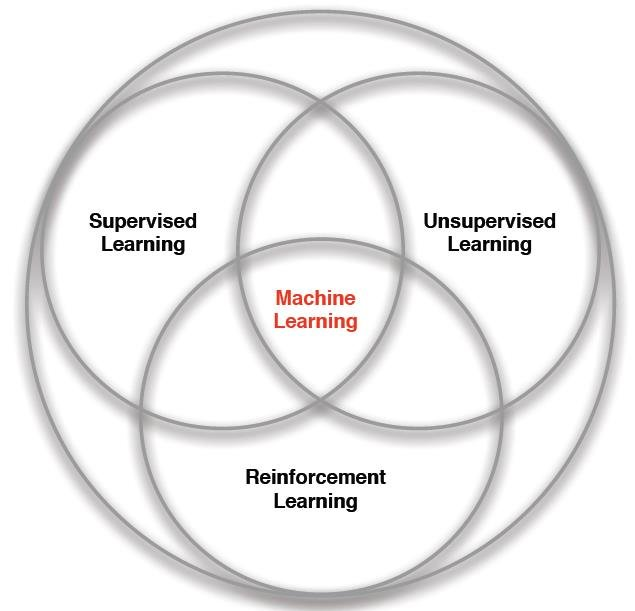
\includegraphics[width=9cm, height=8cm]{MLBranches.PNG}
\end{frame}

\begin{frame}
\frametitle{Overview of the Course}
\pause
\begin{itemize}[<+->]
\item Theory of Markov Decision Processes (MDPs)
\item Dynamic Programming (DP) Algorithms
\item Approximate DP and Backward Induction Algorithms
\item Reinforcement Learning (RL) Algorithms
\item Plenty of Python implementations of models and algorithms
\item Apply these algorithms to 5 Financial/Trading problems:
\begin{itemize}
\item (Dynamic) Asset-Allocation to maximize Utility of Consumption
\item Pricing and Hedging of Derivatives in an Incomplete Market
\item Optimal Exercise/Stopping of Path-dependent American Options
\item Optimal Trade Order Execution (managing Price Impact)
\item Optimal Market-Making (Bids and Asks managing Inventory Risk)
\end{itemize}
\item By treating each of the problems as MDPs (i.e., Stochastic Control)
\item We will go over classical/analytical solutions to these problems
\item Then introduce real-world considerations, and tackle with RL (or DP)
\item Course blends Theory/Math, Algorithms/Coding, Real-World Finance
\end{itemize}
\end{frame}

\begin{frame}
\frametitle{Optimal Asset Allocation to Maximize Consumption Utility}
\pause
\begin{itemize}[<+->]
\item You can invest in (allocate wealth to) a collection of assets
\item Investment horizon is a fixed length of time
\item Each risky asset characterized by a probability distribution of returns
\item Periodically, you are re-allocate your wealth to the various assets
\item Transaction Costs \& Constraints on trading hours/quantities/shorting
\item Allowed to consume a fraction of your wealth at specific times
\item Dynamic Decision: Time-Sequenced Allocation \& Consumption
\item To maximize horizon-aggregated {\em Risk-Adjusted Consumption}
\item {\em Risk-Adjustment} involves a study of {\em Utility Theory}
\end{itemize}
\end{frame}



\begin{frame}
\frametitle{MDP for Optimal Asset Allocation problem}
\pause
\begin{itemize}[<+->]
\item {\em State} is [Current Time, Current Holdings, Current Prices]
\item {\em Action} is [Allocation Quantities, Consumption Quantity]
\item {\em Action}s limited by various real-world trading constraints
\item {\em Reward} is Utility of Consumption less Transaction Costs
\item {\em State}-transitions governed by risky asset movements
\end{itemize}
\end{frame}

\begin{frame}
\frametitle{Derivatives Pricing and Hedging in an Incomplete Market}
\pause
\begin{itemize}[<+->]
\item Classical Pricing/Hedging Theory assumes ``frictionless market''
\item Technically, refered to as \href{https://github.com/coverdrive/technical-documents/blob/master/finance/ArbitrageCompleteness.pdf}{\underline{\textcolor{blue}{arbitrage-free and complete market}}}
\item {\em Complete market} means derivatives can be perfectly replicated
\item But real world has transaction costs and trading constraints
\item So real markets are incomplete where classical theory doesn't fit
\item How to price and hedge in an {\em Incomplete Market}?
\item Maximize ``risk-adjusted-return'' of the derivative plus hedges
\item Similar to Asset Allocation, this is a stochastic control problem
\item Deep Reinforcement Learning helps solve when framed as an MDP 
\end{itemize}
\end{frame}

\begin{frame}
\frametitle{MDP for Pricing/Hedging in an Incomplete Market}
\pause
\begin{itemize}[<+->]
\item {\em State} is [Current Time, PnL, Hedge Qtys, Hedge Prices]
\item {\em Action} is Units of Hedges to be traded at each time step
\item {\em Reward} only at termination, equal to Utility of terminal PnL
\item {\em State}-transitions governed by evolution of hedge prices
\item Optimal Policy $\Rightarrow$ Derivative Hedging Strategy
\item Optimal Value Function $\Rightarrow$ Derivative Price
\end{itemize}
\end{frame}


\begin{frame}
\frametitle{Optimal Exercise of Path-dependent American Options}
\pause
\begin{itemize}[<+->]
\item An American option can be exercised anytime before option maturity
\item Key decision at any time is to exercise or continue
\item The default algorithm is Backward Induction on a tree/grid
\item But it doesn't work for American options with complex payofss 
\item Also, it's not feasible when state dimension is large
\item Industry-Standard: Longstaff-Schwartz's simulation-based algorithm
\item RL is an attractive alternative to Longstaff-Schwartz
\item RL is straightforward once Optimal Exercise is modeled as an MDP
\end{itemize}
\end{frame}

\begin{frame}
\frametitle{MDP for Optimal American Options Exercise}
\pause
\begin{itemize}[<+->]
\item {\em State} is [Current Time, History of Underlying Security Prices]
\item {\em Action} is Boolean: Exercise (i.e., Payoff and Stop) or Continue
\item {\em Reward} always 0, except upon Exercise ($=$ Payoff)
\item {\em State}-transitions governed by Underlying Prices' Stochastic Process
\item Optimal Policy $\Rightarrow$ Optimal Stopping $\Rightarrow$ Option Price
\item Can be generalized to other Optimal Stopping problems
\end{itemize}
\end{frame}

\begin{frame}
\frametitle{Optimal Trade Order Execution (controlling Price Impact)}
\pause
\begin{itemize}[<+->]
\item You are tasked with selling a large qty of a (relatively less-liquid) stock
\item You have a fixed horizon over which to complete the sale
\item Goal is to maximize aggregate sales proceeds over horizon
\item If you sell too fast, {\em Price Impact} will result in poor sales proceeds
\item If you sell too slow, you risk running out of time
\item We need to model temporary and permanent {\em Price Impact}s
\item Objective should incorporate penalty for variance of sales proceeds
\item Again, this amounts to maximizing Utility of sales proceeds
\end{itemize}
\end{frame}

\begin{frame}
\frametitle{MDP for Optimal Trade Order Execution}
\pause
\begin{itemize}[<+->]
\item {\em State} is [Time Remaining, Stock Remaining to be Sold, Market Info]
\item {\em Action} is Quantity of Stock to Sell at current time
\item {\em Reward} is Utility of Sales Proceeds (i.e., Variance-adjusted-Proceeds)
\item {\em Reward} \& {\em State}-transitions governed by {\em Price Impact Model}
\item Real-world {\em Model} can be quite complex ({\em Order Book Dynamics})
\end{itemize}
\end{frame}

\begin{frame}
\frametitle{Optimal Market-Making (controlling Inventory Buildup)}
\pause
\begin{itemize}[<+->]
\item Market-maker's job is to submit bid and ask prices (and sizes)
\item On the Trading {\em Order Book} (which moves due to other players)
\item Market-maker needs to adjust bid/ask prizes/sizes appropriately
\item By anticipating the {\em Order Book Dynamics}
\item Goal is to maximize {\em Utility of Gains} at the end of a suitable horizon
\item If Buy/Sell LOs are too narrow, more frequent but small gains
\item If Buy/Sell LOs are too wide, less frequent but large gains
\item Market-maker also needs to manage potential unfavorable inventory (long or short) buildup and consequent unfavorable liquidation
\item This is a classical stochastic control problem
\end{itemize}
\end{frame}

\begin{frame}
\frametitle{MDP for Optimal Market-Making}
\pause
\begin{itemize}[<+->]
\item {\em State} is [Current Time, Mid-Price, PnL, Inventory of Stock Held]
\item {\em Action} is Bid \& Ask Prices \& Sizes at each time step
\item {\em Reward} is Utility of Gains at termination
\item {\em State}-transitions governed by probabilities of hitting/lifting Bid/Ask
\item Also governed by Order Book Dynamics (can be quite complex)
\end{itemize}
\end{frame}


\begin{frame}
\frametitle{Week by Week (Tentative) Schedule}
\pause
\begin{itemize}[<+->]
\item W1: Markov Decision Processes
\item W2: Bellman Equations \& Dynamic Programming Algorithms
\item W3: Backward Induction and Approximate DP Algorithms
\item W4: Optimal Asset Allocation \& Derivatives Pricing/Hedging
\item W5: Options Exercise,  Order Execution, Market-Making
\item Mid-Term Exam
\item W6: RL For Prediction (MC, TD, TD($\lambda$))
\item W7: RL for Control (SARSA, Q-Learning)
\item W8: Batch Methods (DQN, LSTD/LSPI) and Gradient TD
\item W9: Policy Gradient, Model-based RL, Explore v/s Exploit
\item W10: Read-World RL and Guest Lecture by an Industry leader
\item Final Exam
\end{itemize}
\end{frame}


\begin{frame}
\frametitle{Some Landmark Papers we cover in this course}
\begin{itemize}
\item \href{https://www.jstor.org/stable/1926560}{\underline{\textcolor{blue}{Merton's solution for Optimal Portfolio Allocation/Consumption}}}
\item \href{https://people.math.ethz.ch/~hjfurrer/teaching/LongstaffSchwartzAmericanOptionsLeastSquareMonteCarlo.pdf}{\underline{\textcolor{blue}{Longstaff-Schwartz Algorithm for Pricing American Options}}}
\item \href{https://pdfs.semanticscholar.org/3d2d/773983c5201b58586af463f045befae5bbf2.pdf}{\underline{\textcolor{blue}{Almgren-Chriss paper on Optimal Order Execution}}}
\item \href{https://www.math.nyu.edu/faculty/avellane/HighFrequencyTrading.pdf}{\underline{\textcolor{blue}{Avellaneda-Stoikov paper on Optimal Market-Making}}}
\item \href{https://www.cs.toronto.edu/~vmnih/docs/dqn.pdf}{\underline{\textcolor{blue}{Original DQN paper}}} and \href{https://storage.googleapis.com/deepmind-media/dqn/DQNNaturePaper.pdf}{\underline{\textcolor{blue}{Nature DQN paper}}}
\item \href{http://www.jmlr.org/papers/volume4/lagoudakis03a/lagoudakis03a.pdf}{\underline{\textcolor{blue}{Lagoudakis-Parr paper on Least Squares Policy Iteration}}}
\item \href{http://papers.nips.cc/paper/1713-policy-gradient-methods-for-reinforcement-learning-with-function-approximation.pdf}{\underline{\textcolor{blue}{Sutton, McAllester, Singh, Mansour's Policy Gradient Theorem}}}
\item \href{https://pdfs.semanticscholar.org/a378/b2895a3e3f6a19cdff1a0ad404b301b5545f.pdf}{\underline{\textcolor{blue}{Chang, Fu, Hu, Marcus' AMS origins of Monte Carlo Tree Search}}}
\end{itemize}
\end{frame}


\begin{frame}
\frametitle{Similar Courses offered at Stanford}
\begin{itemize}
\item AA 228/CS 238 (Mykel Kochenderfer)
\item CS 234 (Emma Brunskill)
\item CS 332 (Emma Brunskill)
\item MS\&E 338 (Ben Van Roy)
\item EE 277 (Ben Van Roy)
\item MS\&E 251 (Edison Tse)
\item MS\&E 348 (Gerd Infanger)
\item MS\&E 351 (Ben Van Roy)
\item MS\&E 339 (Ben Van Roy)
\end{itemize}
\end{frame}

\begin{frame}
\frametitle{Salient/Distinguishing features of this Course}
\begin{itemize}[<+->]
\item Emphasis on Foundations and Core Concepts
\item More about {\em why} and {\em how}, versus {\em what}
\item Balance between mathematical precision and intuitive understanding
\item Coding from scratch, avoiding standard packages
\item Encourages {\em Creator/Builder} mindset, versus {\em User} mindset
\item Emphasis on code design driven by mathematical concepts/structures
\item Key purpose of coding: Enables long-term retention of key learnings
\item Several financial trading applications (and a couple from Retail)
\item Coverage of continuous-time versions (elegant, analytical)
\item I will dispel some common myths about industry versus academia
\end{itemize}
\end{frame}

\end{document}
